%===================================== CHAP 2 =================================

\chapter{Neuroscience context}

Before going into the statistics and modeling, it is useful to present some context for the work. The aim of this chapter is to describe the relevant concepts from neuroscience, explain the background for the data material and motivate a practical understanding. Section \ref{NandC} gives a brief description of the signaling and connectivity in neural networks. The source used for this section is the book \textit{Neuroscience}, by Purves. In section \ref{EandA} the hallmarks for Alzheimer's disease in the brain are described. The content is based on sources \cite{Gomez,Witter:2011, Alz}. Section \ref{Lab} provides an outline of the lab experiments where the data material that is background for this project comes from. The information is based on the description of the lab set up in Katrine's master thesis. The same lab set up as will be used for the Alzheimer's experiments. As mentioned in the introduction, only simulated data will be used for analysis in this project. However, the models are developed with these data as background, the idea is that they should also fit to real data. Therefore, these descriptions are included in this project report.  

%En av de som Katrine sendte
%http://www.scholarpedia.org/article/Entorhinal_cortex
%https://en.wikipedia.org/wiki/Entorhinal_cortex


\section{Concepts from neuroscience}


\subsection{Neuron and connections}\\
\label{NandC}
The brain comprise a complex network of neurons that work together by transmitting signals to each other. The basic unit, the neuron, 
 consists of a cell body (soma), an axon and dendrites. Figure \ref{neuron} shows an illustration of a neuron.
\begin{figure}[h]
    \caption{}
    \label{neuron}
    \centering
    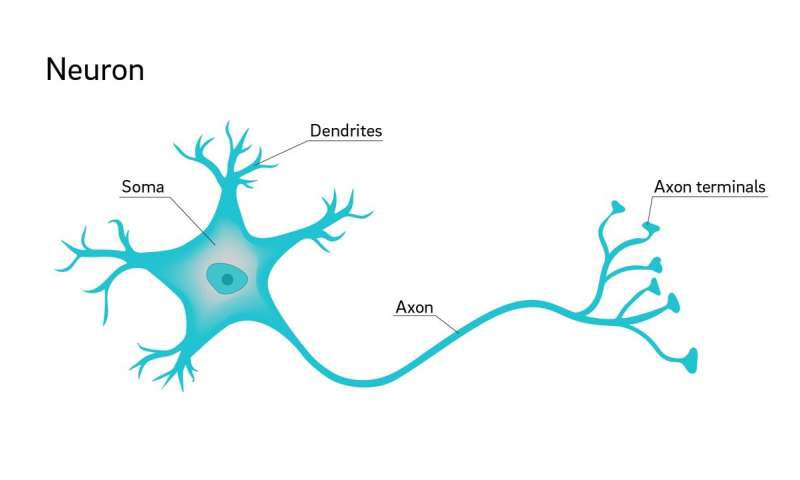
\includegraphics[scale=0.3]{Neuron.jpeg}
\end{figure} 

Neurons can transmit electrical signals to each other through a connection of the axon of one neuron with the dendrite of another. The sending and the receiving neuron are referred to as the "presynaptic neuron" and the "postsynaptic neuron", respectively. Such a connection between two neurons is called a synapse, and is in practice a short gap where chemical units, called neurotransmitters, are allowed to flow from the axon to the dendrite. 

This signaling happens in response to something called an action potential in the presynaptic neuron. When a neuron is at rest, there is a constant potential difference between the inside and the outside of the neuron's cell membrane. An action potential is a rapid increase in this membrane potential, caused by ion flows through channels in the membrane. This action potential then propagates along the axon until it reaches the synapse, and ends up as an electrical signal to the connected neuron. In order for the action potential to occur, the potential difference must reach a certain threshold value. If this threshold is reached, the action potential will take place no matter what. In other words there is an all-or-non property, and if it first takes place the action potential will always have the same strength. This phenomenon is illustrated in figure \ref{AP}. Action potentials will be referred to as neuron firing or spiking.

\begin{figure}[h]
\caption{}
\label{AP}
\begin{subfigure}
\centering
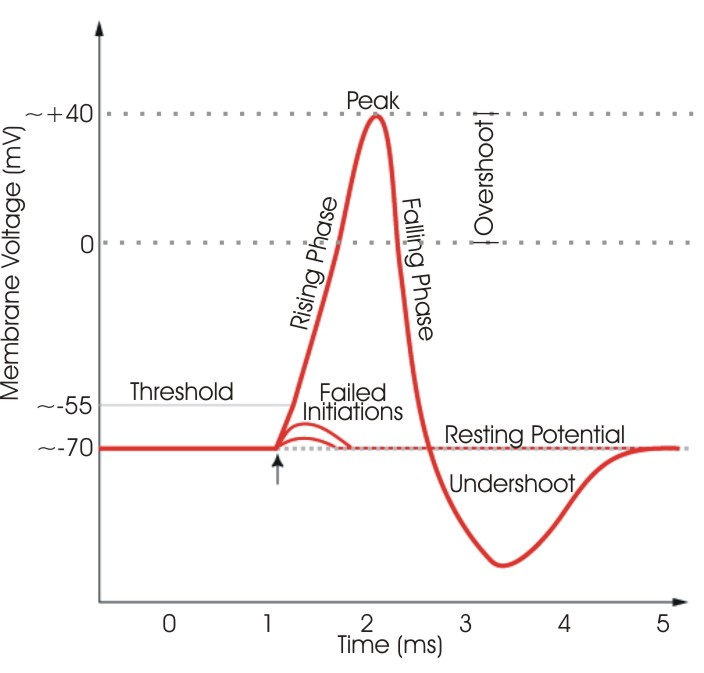
\includegraphics[scale=0.7]{AP.jpg}
\end{subfigure}
\begin{subfigure}
\centering
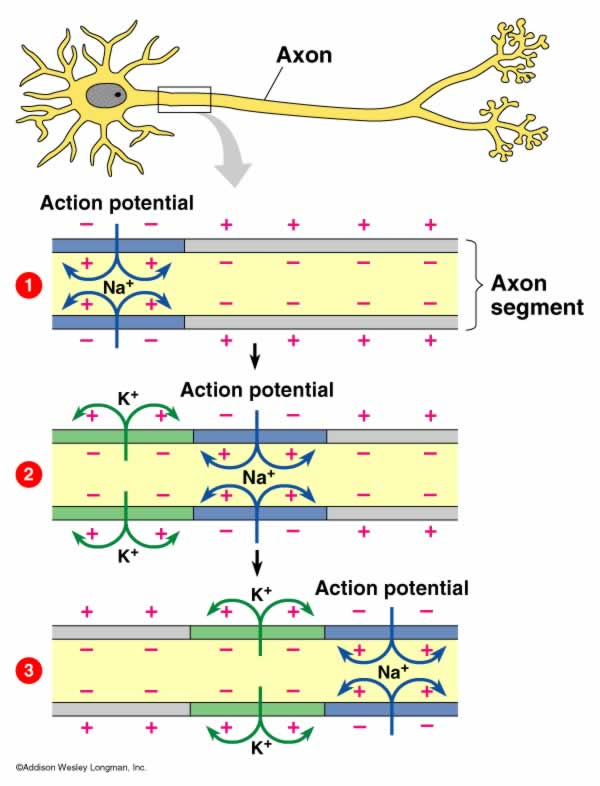
\includegraphics[scale=0.21]{Axjk4.jpg}
\end{subfigure}
\end{figure} 

The developing of an action potential happens in response of some stimuli. This can be external stimuli from some sense, for example a ray of light that hits the eye. Also, action potentials can develop after the receiving of an electrical signal from another neuron. When a signal increase the likelihood of an action potential to also arise in the postsynaptic neuron, this is referred to as an excitatory signal. This enables the possibility for a signal to propagate through the network, and eventually end up for example in a muscle and cause a contraction. On the contrary there are also signals that decrease the chance that the postsynaptic neuron will fire. These are called inhibitory signals.

The  strength of these neural connections are not fixed, but can change over time. A \textit{strong} synapse refers to a high probability that the postsynaptic neuron will be affected by the action potential in the presynaptic neuron. A frequent activation of a synapse can strengthen the synaptic connection. This phenomenon is called "long-term potentiation (LTP) of a synapse. Other times activation of a synapse can weaken the connection over time, known as "long-term depression". These changes of connections are referred to as synaptic plasticity, and is the mechanism that gives rise to learning and memory. \\

\subsection{Entorhinal cortex and Alzheimer's disease}
\label{EandA}

%\begin{itemize}
    %\item More on this section
    %\item Say something about what is known today and what is not. Status of research
    %\item Make connection to the work I am going to do. Why do we think that its an idea to invesigate the learning rule in the context of Alzheimer's research
%\end{itemize}
%The human brain is very good at forgetting. The hippocampus is a structure in the brain that has been associated with various memory functions

The data basis for this project are lab recordings from a part the brain called the entorhinal cortex, which is associated with the earliest indications of AD. The entorhinal cortex is found in the medial temporal lobe and functions as a gateway between the neocortex and the hippocampus. It is a part of the hippocampal memory system (Witter 2011), which is related to declarative memory and learning. The entorhinal cortex is commonly subdivided into six layers, I-VI. Cells in layer II of the entorhinal cortex are shown to be affected in the initial stages of AD, and this part is where the brain tissue for the experiments are extracted from. The position  of the entorhinal cortex in the brain is shown in figure \ref{EC} (left).

\begin{figure}[h]
    \caption{(Left) Illustration of brain showing location of the Entorhinal cortex. (Right) Visual comparison of healthy brain and brain with Alzheimer's disease.}
    \label{EC}
    \centering
    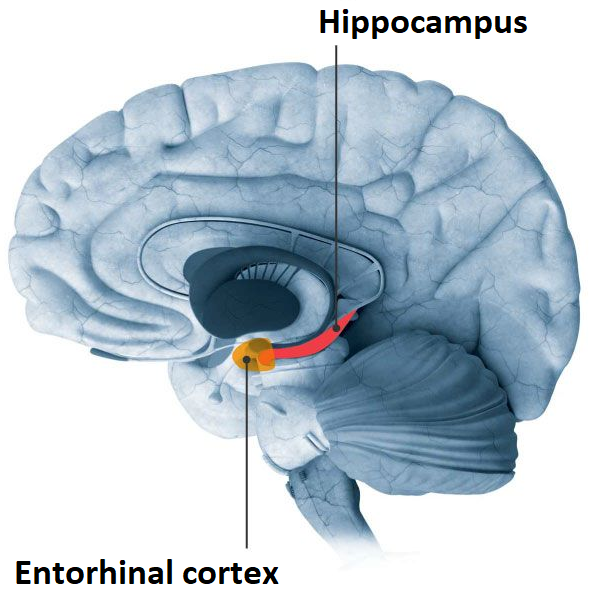
\includegraphics[scale=0.35]{Entorhinal_cortex2.png}
    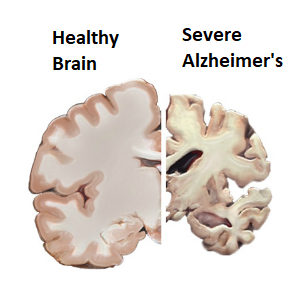
\includegraphics[scale=0.8]{fig/Alzheimers_picture.png}    
    \label{brain}
\end{figure} 

Characteristic to brains with Alzheimer's is loss of synapses and neurons. When a patient have struggled from AD for a long time, it is easily seen that the brain has shrinked significantly. Figure \ref{EC} (right) illustrates how a brain can look like after having AD for many years. Exactly what causes these losses is still not known, but it is assumed that the accumulation of some protein types called amyloid plaques and neurofirbillary tangles are involved. These changes in the brain begin many years before behavioural symptoms occur. However, if we hope for a treatment of the AD a critical step is to detect these changes when they start, before the disease have had the chance to damage the brain.




%The entorhinal cortex (EC) is an area of the brain located in the medial temporal lobe and functions as a hub in a widespread network for memory, navigation and the perception of time.[1] The EC is the main interface between the hippocampus and neocortex.  The entorhinal cortex (EC), in particular (Wikipedia)
%the layer II of the domains located towards the collateral/rhinal fissure, contains neurons that are
%among the very first to undergo pathological alterations associated with the disease. Specifically,
%neurons in this domain develop the initial cortical tau pathology, while layer II is also known to
%exhibit severe neuronal loss already during the pre-clinical stages of AD. Furthermore, layer IIneurons are also subject to early accumulation of intracellular Aβ. In order to help enable the study
%of these early neuronal pathologies the work in this thesis was aimed at developing a platform for
%studying the LEC layer II neuronal population in vitro. (Katrines master)

\section{Data material}

\label{Lab}\\
The data material that is the background for this project is electric potential recordings from neurons in mouse brains with and without AD. Mice do not get Alzheimer's naturally, so AD mice are constructed with a genetic mutation that gives rise to amyloid plaque accumulations in their brains. It is demonstrated that at an age of 8 months, mice with this mutation have learning impairments and behavioural differences from healthy mice (\cite{Radde}). 

Tissue from layer II of the entorhinal cortex is gathered by microdissection from the mouse brains (\cite{Katrine}). Microelectrode arrays, a sheet of equally spaced needle electrodes, are put into the brain tissue. One electrode can measure the electrical activity of one neuron over time interval $[0,T]$. When a neuron undergoes an action potential, this will appear as a peak in these recordings. It is the time points for these action potentials that are of interest, and not the actual voltage values. Let's label the N recorded neurons with numbers $1,2,...,N$. Hence, the relevant data material is a sequence of recorded time points for the action potentials for each neuron,
\begin{equation}
    \{\{a_i\}\}_{i=1}^{N} = \{a_{i1}, a_{i2}, ...\}_{i=1}^{N} \quad a_{ix} \in [0,T]
\end{equation}

where $a_{ix}$ is the recorded time for the x'th action potential for neuron $i$, and $a_{ix-1} < a_{ix}$. Such a sequence of time stamps for neuron firing is called a spike train.\\







\cleardoublepage